\documentclass[10pt,leqno]{article}

\usepackage[%
  tmargin=1.2in,bmargin=1.2in,%
  lmargin=1.8in,rmargin=1.8in,%
]{geometry}
\usepackage{fancyhdr}
\usepackage{titlesec}
\usepackage{appendix}
\usepackage{microtype}
\usepackage[hyphens]{url}
\usepackage{enumitem}
\usepackage{xspace}
\usepackage{etoolbox}
\usepackage{ifthen}
\usepackage{tikz}
\usepackage{tikz-cd}

\usepackage{amsmath}
\definecolor{darkred}{rgb}{0.5,0.0,0.0}
\usepackage[%
  colorlinks,%
  linkcolor=darkred,%
  citecolor=darkred,%
  urlcolor=darkred,%
]{hyperref}
\usepackage{amsthm,amssymb}
% \usepackage[lining,semibold]{libertine}
% \usepackage{textcomp,stmaryrd}
% \usepackage[libertine,cmintegrals,bigdelims]{newtxmath}
% \useosf
% \usepackage[%
%   cal=boondox, calscaled=0.97,%
%   bb=boondox, bbscaled=0.98,%
% ]{mathalfa}
\usepackage{cleveref}

\frenchspacing
\urlstyle{rm}

\AtBeginDocument{%
  \setlength{\abovedisplayskip}{1.5ex plus 0.3ex minus 0.3ex}%
  \setlength{\abovedisplayshortskip}{1.0ex plus 0.3ex minus 0.3ex}%
  \setlength{\belowdisplayskip}{1.5ex plus 0.3ex minus 0.3ex}%
  \setlength{\belowdisplayshortskip}{1.0ex plus 0.3ex minus 0.3ex}%
}

\let\theoldbibliography\thebibliography
\renewcommand{\thebibliography}[1]{%
  \theoldbibliography{#1}%
  \setlength{\parskip}{0ex}
  \setlength{\itemsep}{0.5ex plus 0.2ex minus 0.2ex}
  \small
}

\pagestyle{fancy}
\renewcommand{\headrulewidth}{0pt}
\renewcommand{\footrulewidth}{0pt}
\fancyhf{}
\fancyfoot[C]{\small\thepage}

\renewcommand{\title}[1]{\newcommand{\thetitle}{#1}}
\renewcommand{\author}[1]{\newcommand{\theauthor}{#1}}
\renewcommand{\date}[1]{\newcommand{\thedate}{#1}}

\renewcommand{\maketitle}{%
  \begin{center}
    {\bfseries\MakeUppercase{%
      \thetitle}}\\[2.5ex]
    {\footnotesize\MakeUppercase{%
      \theauthor}}\\[2.5ex]
    \ifthenelse{\equal{\thedate}{}}{}{%
      \small%
      \setlength{\tabcolsep}{0.2em}%
      \begin{tabular}{rl}
        original: & \thedate \\
        updated: & \today
      \end{tabular}
    }
  \end{center}
  \vspace{2.5ex}
  \thispagestyle{fancy}
}

%%%%%%%%%%%%%%%%%%%%%%%%%%%%%%%%%%%%%%%%%%%%%%%%%%%%%%%%%%%%%%%%%%%%%%

\cspreto{section}{\setcounter{equation}{0}}

\titleformat{\section}{\centering\scshape}{\thesection.}{0.4em}{}
\titlespacing{\section}{0pt}{*4}{*1}
\titleformat{\subsection}{\scshape}{\thesubsection.}{0.4em}{}
\titlespacing{\subsection}{0pt}{*2.5}{*1}

% Display format for equations
\newcommand{\crefeqfmt}[1]{
  \crefformat{#1}{(##2##1##3)}
  \Crefformat{#1}{(##2##1##3)}
  \crefrangeformat{#1}{(##3##1##4--##5##2##6)}
  \Crefrangeformat{#1}{(##3##1##4--##5##2##6)}
  \crefmultiformat{#1}{(##2##1##3}{, ##2##1##3)}{, ##2##1##3}{, ##2##1##3)}
  \Crefmultiformat{#1}{(##2##1##3}{, ##2##1##3)}{, ##2##1##3}{, ##2##1##3)}
  \crefrangemultiformat{#1}{(##3##1##4--##5##2##6}{, ##3##1##4--##5##2##6)}{, ##3##1##4--##5##2##6}{, ##3##1##4--##5##2##6)}
  \Crefrangemultiformat{#1}{(##3##1##4--##5##2##6}{, ##3##1##4--##5##2##6)}{, ##3##1##4--##5##2##6}{, ##3##1##4--##5##2##6)}
}
% Display format for sections
\newcommand{\crefsecfmt}[1]{%
  \crefformat{#1}{\S##2##1##3}
  \Crefformat{#1}{\S##2##1##3}
  \crefrangeformat{#1}{\S\S##3##1##4--##5##2##6}
  \Crefrangeformat{#1}{\S\S##3##1##4--##5##2##6}
  \crefmultiformat{#1}{\S\S##2##1##3}{ and~##2##1##3}{, ##2##1##3}{ and~##2##1##3}
  \Crefmultiformat{#1}{\S\S##2##1##3}{ and~##2##1##3}{, ##2##1##3}{ and~##2##1##3}
  \crefrangemultiformat{#1}{\S\S##3##1##4--##5##2##6}{ and~##3##1##4--##5##2##6}{, ##3##1##4--##5##2##6}{ and~##3##1##4--##5##2##6}
  \Crefrangemultiformat{#1}{\S\S##3##1##4--##5##2##6}{ and~##3##1##4--##5##2##6}{, ##3##1##4--##5##2##6}{ and~##3##1##4--##5##2##6}
}
\crefeqfmt{equation}
\crefeqfmt{enumi}
\crefeqfmt{enumii}
\crefsecfmt{section}
\crefsecfmt{subsection}
\crefsecfmt{appendix}
\crefname{part}{Part}{Parts}
\crefname{chapter}{Chapter}{Chapters}
\crefname{figure}{Figure}{Figures}

\makeatletter

\newcommand{\thmnumfont}{\bfseries}
\newcommand{\thmheadfont}{\bfseries}
\newcommand{\thmnotefont}{\bfseries}
\newcommand{\thmhorizspace}{0.4em}

\def\swappedhead#1#2#3{%
  \thmnumber{\@upn{{\thmnumfont#2}}\@ifnotempty{#1}{.\hspace{0.25em}}}%
  \thmheadfont\thmname{#1}%
  \@ifnotempty{#3}{\ \thmnote{\thmnotefont(#3)}}%
}
\swapnumbers

\newtheoremstyle{block}%
  {2.0ex plus 0.2ex minus 0.1ex}% Space above
  {2.0ex plus 0.2ex minus 0.1ex}% Space below
  {} % Body font
  {} % Indent amount
  {\thmheadfont} % Theorem head font
  {.} % Punctuation after theorem head
  {\thmhorizspace} % Space after theorem head
  {} % Theorem head spec (can be left empty, meaning ‘normal’)

\renewenvironment{proof}[1][Proof]{\par
  \pushQED{\qed}%
  \normalfont%
  \topsep1ex plus 0.2ex minus 0.1ex\relax%
  \labelsep \thmhorizspace\relax%
  \trivlist
  \item[\hskip\labelsep\thmheadfont
    #1\@addpunct{.}]\ignorespaces
}{%
  \popQED\endtrivlist\@endpefalse%
}

\makeatother

\theoremstyle{block}

\newcommand{\defthm}[2]{%
  \newtheorem{#1}[equation]{#2}%
  \crefeqfmt{#1}%
  \newtheorem*{#1*}{#2}%
}

\defthm{algorithm}{Algorithm}
\defthm{conjecture}{Conjecture}
\defthm{construction}{Construction}
\defthm{convention}{Convention}
\defthm{corollary}{Corollary}
\defthm{definition}{Definition}
\defthm{definitions}{Definitions}
\defthm{example}{Example}
\defthm{examples}{Examples}
\defthm{exercise}{Exercise}
\defthm{fact}{Fact}
\defthm{intuition}{Intuition}
\defthm{lemma}{Lemma}
\defthm{notation}{Notation}
\defthm{nothing}{}
\defthm{proposition}{Proposition}
\defthm{question}{Question}
\defthm{remark}{Remark}
\defthm{remarks}{Remarks}
\defthm{situtation}{Situation}
\defthm{theorem}{Theorem}

\setlist{%
  leftmargin=2.5em, parsep=0ex, listparindent=\parindent,
  itemsep=1.0ex, topsep=1.0ex,%
}

\setlist[enumerate, 1]{%
  label=(\alph*),%
  ref=\alph*,%
  widest=d,%
}
\setlist[enumerate, 2]{%
  label=(\roman*),%
  ref=\theenumi.\roman*,%
}
\setlist[itemize, 1]{%
  label=$\vcenter{\hbox{\footnotesize$\bullet$}}$,%
}
\setlist[itemize, 2]{label=--}

%%%%%%%%%%%%%%%%%%%%%%%%%%%%%%%%%%%%%%%%%%%%%%%%%%%%%%%%%%%%%%%%%%%%%%

\makeatletter

\let\ea\expandafter

\newcount\foreachcount

\def\foreachletter#1#2#3{\foreachcount=#1
  \ea\loop\ea\ea\ea#3\@alph\foreachcount
  \advance\foreachcount by 1
  \ifnum\foreachcount<#2\repeat}

\def\foreachLetter#1#2#3{\foreachcount=#1
  \ea\loop\ea\ea\ea#3\@Alph\foreachcount
  \advance\foreachcount by 1
  \ifnum\foreachcount<#2\repeat}

% Roman: \rA is \mathrm{A}
\def\definerm#1{%
  \ea\gdef\csname r#1\endcsname{\ensuremath{\mathrm{#1}}\xspace}}
\foreachLetter{1}{27}{\definerm}
\foreachletter{1}{27}{\definerm}
% Script: \sA is \mathscr{A}
\def\definescr#1{%
  \ea\gdef\csname s#1\endcsname{\ensuremath{\mathscr{#1}}\xspace}}
\foreachLetter{1}{27}{\definescr}
% Calligraphic: \cA is \mathcal{A}
\def\definecal#1{%
  \ea\gdef\csname c#1\endcsname{\ensuremath{\mathcal{#1}}\xspace}}
\foreachLetter{1}{27}{\definecal}
% Bold: \bA is \mathbf{A}
\def\definebold#1{%
  \ea\gdef\csname b#1\endcsname{\ensuremath{\mathbf{#1}}\xspace}}
\foreachLetter{1}{27}{\definebold}
% Blackboard Bold: \lA is \mathbb{A}
\def\definebb#1{%
  \ea\gdef\csname l#1\endcsname{\ensuremath{\mathbb{#1}}\xspace}}
\foreachLetter{1}{27}{\definebb}
% Fraktur: \ka is \mathfrak{a}, \kA is \mathfrak{A}
\def\definefrak#1{%
  \ea\gdef\csname k#1\endcsname{\ensuremath{\mathfrak{#1}}\xspace}}
\foreachletter{1}{27}{\definefrak}
\foreachLetter{1}{27}{\definefrak}
% Sans serif: \iA \is \mathsf{A}
\def\definesf#1{%
  \ea\gdef\csname i#1\endcsname{\ensuremath{\mathsf{#1}}\xspace}}
\foreachletter{1}{6}{\definesf}
\foreachletter{7}{14}{\definesf}
\foreachletter{15}{27}{\definesf}
\foreachLetter{1}{27}{\definesf}
% Bar: \Abar is \overline{A}, \abar is \overline{a}
\def\definebar#1{%
  \ea\gdef\csname #1bar\endcsname{\ensuremath{\overline{#1}}\xspace}}
\foreachLetter{1}{27}{\definebar}
\foreachletter{1}{8}{\definebar} % \hbar is something else!
\foreachletter{9}{15}{\definebar} % \obar is something else!
\foreachletter{16}{27}{\definebar}
% Tilde: \Atil is \widetilde{A}, \atil is \widetilde{a}
\def\definetil#1{%
  \ea\gdef\csname #1til\endcsname{\ensuremath{\widetilde{#1}}\xspace}}
\foreachLetter{1}{27}{\definetil}
\foreachletter{1}{27}{\definetil}
% Hats: \Ahat is \widehat{A}, \ahat is \widehat{a}
\def\definehat#1{%
  \ea\gdef\csname #1hat\endcsname{\ensuremath{\widehat{#1}}\xspace}}
\foreachLetter{1}{27}{\definehat}
\foreachletter{1}{27}{\definehat}
% Checks: \Achk is \widecheck{A}, \achk is \widecheck{a}
\def\definechk#1{%
  \ea\gdef\csname #1chk\endcsname{\ensuremath{\widecheck{#1}}\xspace}}
\foreachLetter{1}{27}{\definechk}
\foreachletter{1}{27}{\definechk}
% Underline: \Aund is \underline{A}, \aund is \underline{a}
\def\defineul#1{%
  \ea\gdef\csname #1und\endcsname{\ensuremath{\underline{#1}}\xspace}}
\foreachLetter{1}{27}{\defineul}
\foreachletter{1}{27}{\defineul}

\makeatother

%%%%%%%%%%%%%%%%%%%%%%%%%%%%%%%%%%%%%%%%%%%%%%%%%%%%%%%%%%%%%%%%%%%%%%

\usetikzlibrary{calc,decorations.pathmorphing,shapes,arrows}
\tikzcdset{
  arrow style=tikz,
  diagrams={>={stealth}},
}

\newcommand{\arrlen}{1em}
\renewcommand{\to}{\mathrel{\tikz[baseline]%
    \draw[>=stealth,->](0,0.5ex)--(\arrlen,0.5ex);}}
\newcommand{\from}{\mathrel{\tikz[baseline]%
    \draw[>=stealth,<-](0,0.5ex)--(\arrlen,0.5ex);}}
\renewcommand{\mapsto}{\mathrel{\tikz[baseline]%
    \draw[>=stealth,|->](0,0.5ex)--(\arrlen,0.5ex);}}
\newcommand{\inj}{\mathrel{\tikz[baseline]%
    \draw[>=stealth,right hook->](0,0.5ex)--(\arrlen,0.5ex);}}
\newcommand{\surj}{\mathrel{\tikz[baseline]%
    \draw[>=stealth,->>](0,0.5ex)--(\arrlen,0.5ex);}}
\newcommand{\fromto}{\mathrel{%
  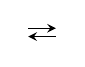
\begin{tikzpicture}[baseline]%
    \draw[>=stealth,<-](0,0.15ex)--(\arrlen,0.15ex);%
    \draw[>=stealth,->](0,0.85ex)--(\arrlen,0.85ex);%
  \end{tikzpicture}}}
\newcommand{\doubto}{\mathrel{%
  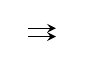
\begin{tikzpicture}[baseline]%
    \draw[>=stealth,->](0,0.15ex)--(\arrlen,0.15ex);%
    \draw[>=stealth,->](0,0.85ex)--(\arrlen,0.85ex);%
  \end{tikzpicture}}}
\newcommand{\lblto}[1]{\mathrel{%
    \begin{tikzpicture}[baseline= {( $ (current bounding box.south) + (0,-0.5ex) $ )}]
      \node[inner sep=.4ex] (a) {\,$\scriptstyle #1$\,};
      \draw[>=stealth,->] (a.south west) -- (a.south east);
    \end{tikzpicture}}}
\newcommand{\isoto}{\lblto{\sim}}

\newcommand{\simpl}[3]{
  \begin{tikzcd}[ampersand replacement=\&, column sep=small]
    #1 \&
    #2 \ar[l, shift right=0.35ex]
       \ar[l, shift left=0.35ex] \&
    #3 \ar[l, shift right=0.70ex]
       \ar[l, shift left=0.70ex]
       \ar[l] \&
    \cdots \ar[l, shift right=0.35ex]
           \ar[l, shift left=0.35ex]
           \ar[l, shift right=1.05ex]
           \ar[l, shift left=1.05ex]
  \end{tikzcd}
}
\newcommand{\cosimpl}[3]{
  \begin{tikzcd}[ampersand replacement=\&, column sep=small]
    #1 \ar[r, shift right=0.35ex]
       \ar[r, shift left=0.35ex] \&
    #2 \ar[r, shift right=0.70ex]
       \ar[r, shift left=0.70ex]
       \ar[r] \&
    #3 \ar[r, shift right=0.35ex]
       \ar[r, shift left=0.35ex]
       \ar[r, shift right=1.05ex]
       \ar[r, shift left=1.05ex] \&
    \cdots
  \end{tikzcd}
}

\newcommand{\tto}{\mathrel{\tikz[baseline]%
    \draw[>=stealth,->,double, double distance = 0.3ex](0,0.5ex)--(\arrlen,0.5ex);}}
\newcommand{\doubfrom}{\mathrel{%
  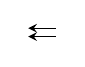
\begin{tikzpicture}[baseline]%
    \draw[>=stealth,<-](0,0.15ex)--(\arrlen,0.15ex);%
    \draw[>=stealth,<-](0,0.85ex)--(\arrlen,0.85ex);%
  \end{tikzpicture}}}
\newcommand{\tripfrom}{\mathrel{%
  
\begin{tikzpicture}[baseline]%
    \draw[>=stealth,<-](0,0.00ex)--(\arrlen,0.00ex);%
    \draw[>=stealth,<-](0,0.50ex)--(\arrlen,0.50ex);%
    \draw[>=stealth,<-](0,1.00ex)--(\arrlen,1.00ex);%
  \end{tikzpicture}}}


\renewcommand{\l}{\left}
\renewcommand{\r}{\right}
\newcommand{\f}{\frac}
\renewcommand{\o}{\overline}
\renewcommand{\u}{\underline}
\newcommand{\til}{\widetilde}
\renewcommand{\hat}{\widehat}
\newcommand{\del}{\partial}
\newcommand{\dash}{\text{-}}
\renewcommand{\c}{\colon}
\newcommand{\lc}{\,:\!}
\newcommand{\ce}{\coloneq}%{\mathrel{:=}}
\newcommand{\ec}{\eqcolon}%{\mathrel{=:}}
\newcommand{\iso}{\simeq}
\newcommand{\dual}{\vee}
\newcommand{\ldb}{\llbracket}
\newcommand{\rdb}{\rrbracket}

\newcommand{\Obj}{\operatorname{Obj}}
\newcommand{\Hom}{\operatorname{Hom}}
\newcommand{\Map}{\operatorname{Map}}
\newcommand{\Fun}{\operatorname{Fun}}
\newcommand{\Aut}{\operatorname{Aut}}
\newcommand{\Iso}{\operatorname{Iso}}
\renewcommand{\id}{\mathrm{id}}
\renewcommand{\im}{\operatorname{im}}
\newcommand{\op}{\mathrm{op}}
\newcommand{\univ}{\mathrm{univ}}
\newcommand{\colim}{\operatorname*{colim}}
\newcommand{\dlim}{\displaystyle\lim}
\newcommand{\dcolim}{\displaystyle\colim}
\newcommand{\Spec}{\operatorname{Spec}}
\newcommand{\Spf}{\operatorname{Spf}}

%%%%%%%%%%%%%%%%%%%%%%%%%%%%%%%%%%%%%%%%%%%%%%%%%%%%%%%%%%%%%%%%%%%%%%


\title{The Yoneda lemma}
\author{Arpon Raksit}
\date{November 6, 2013}

\numberwithin{equation}{section}
% \cspreto{section}{\setcounter{equation}{0}}

\begin{document}
\maketitle
\thispagestyle{fancy}

%%%%%%%%%%%%%%%%%%%%%%%%%%%%%%%%%%%%%%%%%%%%%%%%%%%%%%%%%%%%%%%%%%%%%%

\newcommand{\C}{\mathcal{C}}
\newcommand{\Set}{\mathrm{Set}}
\newcommand{\PSh}{\mathrm{PSh}}

\section{Introduction}

This is going to be short. I feel like every so often I realise how
magical the Yoneda lemma is. One of those realisations just occurred
so let me write something down. I'll record the statement and proof of
the lemma here too, for completeness.

\begin{notation}
  We fix throughout a (locally small) category $\C$. Denote by
  $\PSh(\C)$ the category of (contravariant) functors $\C^{\op} \to
  \Set$.
\end{notation}

\begin{definition}
  For $X \in \Obj(\C)$ we define the functor $h_X : \C^{\op} \to \Set$
  by:
  \begin{itemize}
  \item $h_X(T) \ce \Hom_\C(T,X)$ for $T \in \Obj(\C)$;
  \item $h_X(f) : h_X(T) \to h_X(S)$ sends $g \in \Hom_\C(T,X) \mapsto
    g \circ f \in \Hom_\C(S,X)$ for $f \in \Hom_\C(S,T)$.
  \end{itemize}
  Observe also that any $f \in \Hom_\C(X,Y)$ defines a natural
  transformation $h_f : h_X \to h_Y$ by $g \in \Hom_\C(T,X) \mapsto f
  \circ g \in \Hom_\C(T,Y)$. Thus we have defined a functor $h : \C
  \to \PSh(\C)$.
\end{definition}

\begin{lemma}[Yoneda]
  Let $F : \C^{\op} \to \Set$ any (contravariant) functor. Let $X \in
  \Obj(C)$. Then there is a natural bijection
  \[
  \Hom_{\PSh(\C)}(h_X,F) \simeq F(X)
  \]
  between the natural transformations $h_X \to F$ and the set $F(X)$.
\end{lemma}

\begin{proof}
  Let $\alpha : h_X \to F$ a natural transformation. Then for each $T
  \in \Obj(\C)$ and $f \in \Hom_\C(T,X)$, by definition of $h$ we have
  the commutative diagram
  \[
  \begin{tikzcd}[column sep = large]
    \Hom_\C(X,X) \rar{g \mapsto g \circ f} \dar{\alpha_x} &
    \Hom_\C(T,X) \dar{\alpha_T} \\ F(X) \rar{F(f)} & F(T).
  \end{tikzcd}
  \]
  Setting $g = \id_X$ gives us that $\alpha_T(f) =
  F(f)(\alpha_X(\id_X))$. It follows that
  \[
  \Hom_{\PSh(\C)}(h_X, F) \to F(X), \quad \alpha \mapsto
  \alpha_X(\id_X)
  \]
  gives the necessary bijection.
\end{proof}

\begin{corollary}
  \label{yoneda-embedding}
  The functor $h : \C \to \PSh(\C)$ is fully faithful. In particular, $X
  \simeq Y$ if and only if $h_X \simeq h_Y$ for $X,Y \in \Obj(\C)$.
\end{corollary}

\begin{proof}
  Setting $F \ce h_Y$ in the Yoneda lemma above gives us
  precisely that the map $\Hom_\C(X,Y) \to \Hom_{\PSh(\C)}(h_X,h_Y)$
  induced by $h$ is a bijection.
\end{proof}

\begin{remark}
  In light of (\ref{yoneda-embedding}), we call $h$ the \textit{Yoneda
    embedding}.
\end{remark}

%%%%%%%%%%%%%%%%%%%%%%%%%%%%%%%%%%%%%%%%%%%%%%%%%%%%%%%%%%%%%%%%%%%%%%

\section{Some magic}

We review the notion of a fibre product, the discussion of which in
\cite{gortzwedhorn} being what prompted these notes in the first
place. Throughout we let $u : X \to S$ and $v : Y \to S$ two morphisms
in $\C$.

\begin{definition}
The \textit{fibre product of $X$ and $Y$ over $S$} is an object $X
\times_S Y \in \Obj(\C)$ equipped with \textit{projections} $p : X
\times_S Y \to X$ and $q : X \times_S Y \to Y$ satisfying:
\begin{enumerate}
\item $u \circ p = v \circ q$, and
\item for any $T \in \Obj(\C)$ and morphisms $a : T \to X$ and $b : T
  \to Y$ such that $u \circ a = v \circ b$, there exists a unique
  morphism $a \times b : T \to X \times_S Y$ such that $a = p \circ (a
  \times b)$ and $b = q \circ (a \times b)$.
\end{enumerate}
This is encapuslated by the following diagram:
\[
\begin{tikzcd}
  T \ar[bend left]{rrd}{b} \ar[bend right]{ddr}{a}
  \ar[dashed]{dr}{\exists!\, a \times b} & & \\ & X \times_S Y \rar{q}
  \dar{p} & Y \dar{v} \\ & X \rar{u} & S.
\end{tikzcd}
\]
For the usual reasons, this characterises $X \times_S Y$ up to
(unique) isomorphism.

One more bit of terminology: if we have the data in (2) such that $c$
is moreover an isomorphism---that is, $T$ equipped with $a,b$ is in
fact a fibre product of $X$ and $Y$ over $S$---we say the commutative
square
\[
\begin{tikzcd}
  T \rar{b} \dar{a} & Y \dar{v} \\ X \rar{u} & S
\end{tikzcd}
\]
is \textit{cartesian}, or a \textit{pullback diagram}.
\end{definition}

\begin{example}
  It is easy to see that fibre products exist in the category
  $\Set$. Indeed, they're exactly what you expect them to be (check
  that this construction satisfies the universal property above):
  \[
  X \times_S Y \simeq \{(x, y) \mid x \in X, y \in Y, u(x) = v(y)\}.
  \]
  On the other hand, it can be much more difficult to understand fibre
  products in other categories in this concrete set-theoretic manner
  (e.g., the category of schemes, where fibre products are incredibly
  prevalent). Indeed, as with other universal constructions, it is
  often much easier to work with the fibre product abstractly. But
  here's another way to work with it: the Yoneda embedding magically
  lets us reduce things to the familiar category $\Set$!  Let's see
  what I mean.
\end{example}

\begin{lemma}
  \label{magic}
  An object $Z \in \Obj(\C)$ equipped with $p : Z \to X$ and $q : Z \to
  Y$ is a fibre product of $X$ and $Y$ over $S$ if and only if the
  diagram (in the category $\Set$)
  \[
  \begin{tikzcd}
    \Hom_\C(T, Z) \rar{h_q} \dar{h_p} & \Hom_\C(T, Y) \dar{h_v}
    \\ \Hom_\C(T,X) \rar{h_u} & \Hom_\C(T,S).
  \end{tikzcd}
  \]
  is commutative and cartesian, i.e., for all $T \in \Obj(\C)$ we have
  \[
  \Hom_\C(T,Z) \simeq \Hom_\C(T,X) \times_{\Hom_\C(T,S)}
  \Hom_\C(T,Y).
  \]
\end{lemma}

\begin{proof}
  The condition that the diagram commutes is equivalent to the
  condition that $u \circ p = v \circ q$ since the Yoneda embedding is
  fully faithful. And, just by staring at things for long enough, we
  see that saying
  \begin{align*}
  \Hom_\C(T,Z) &\simeq \Hom_\C(T,X) \times_{\Hom_\C(T,S)} \Hom_\C(T,Y)
  \\ &\simeq \{(a, b) \mid a : T \to X, b : T \to Y, u \circ a = v
  \circ b\}
  \end{align*}
  is equivalent to saying that $Z$ satisfies the necessary universal
  property.
\end{proof}

\begin{remark}
  The above lemma is a great example of a tautology, albeit wrapped in
  formalism. The point is that saying we have a cartesian square in
  $\C$ and saying the Yoneda embedding of the square is cartesian in
  $\Set$ are really precisely the same statement: to give a map into
  $X \times_S Y$ is to give maps into $X$ and $Y$ which induce the
  same map into $S$.
\end{remark}

Ok, so that's what I mean when I say the Yoneda embedding reduces us
to talking about sets. Let's see it in action (briefly).

\begin{lemma}
  For all morphisms $S \to T$ the diagram
  \[
  \begin{tikzcd}
    X \times_S Y \rar{p \times q} \ar{d}[left]{u \circ p = v \circ q}
    & X \times_T Y \dar{u \times v} \\ S \rar{\id_S \times \id_S} & S
    \times_T S
  \end{tikzcd}
  \]
  is commutative and cartesian, assuming all the fibre products
  written exist. That is, $X \times_S Y \simeq S \times_{S \times_T S}
  (X \times_T Y)$.
\end{lemma}

\begin{proof}
  We are reduced to the case that $\C = \Set$ immediately by
  (\ref{magic})! In this case, as you can check, our concrete
  description of the fibre product makes the claim obvious!
\end{proof}

Observe that this last proof was two sentences, each ending with an
exclamation point. I seriously feel like this Yoneda trick is magic
here. Sure, one can argue completely abstractly using only the
universal properties of all the fibre products written down---that's
how I proved this the first time I saw it---but this is just so much
cleaner and intuitive, I think!

\begin{remark}
  As an aside, this last lemma is actually pretty useful. It implies
  for instance in the category of schemes that if $S \to T$ is
  separated then, by stability under base change, $X \times_S Y \to X
  \times_T Y$ (note the graph morphism is a special case of this) is a
  closed immersion.
\end{remark}

%%%%%%%%%%%%%%%%%%%%%%%%%%%%%%%%%%%%%%%%%%%%%%%%%%%%%%%%%%%%%%%%%%%%%%

\bibliographystyle{amsalpha}
\bibliography{/Users/arpon/Documents/grain/refs/math}

\end{document}
